%%%%%%%%%%%%%%%%%%%%%%%%%%%%%%%%%%%%%%%%%%%%%%%%%%%%%%%%%%%%%%%%%%%%%%%%
%                                                                      %
%     File: IST_Report_Architecture.tex                                    %
%                                                                      %
%%%%%%%%%%%%%%%%%%%%%%%%%%%%%%%%%%%%%%%%%%%%%%%%%%%%%%%%%%%%%%%%%%%%%%%%
% !TEX root = IST_Report.tex
\clearpage

\chapter{Arquitectura}
\label{chapter:architecture}
Neste capítulo é apresentada a arquitectura do sistema, a interligação entre os vários módulos e uma explicação  detalhada do funcionamento dos vários procedimentos como a cifra e assinatura.
% ----------------------------------------------------------------------
\section{Visão Geral}
\label{section:estrutura}
A solução desenvolvida permite a troca de mensagens de modo seguro e com garantias temporais. Esta solução é constituída por 3 módulos: Sender, Receiver e um servidor de Timestamp (\textbf{Figura~\ref{fig:chart}}).\\

\begin{figure}[htp]
\centering 
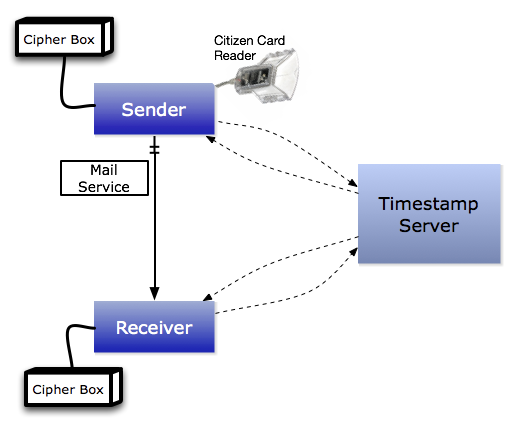
\includegraphics[width=12cm]{./Figures/chart.png}
\caption{Arquitectura do Sistema}
\label{fig:chart}
\end{figure}

O Sender pretende enviar um conjunto de dados para o Receiver mas com garantias de \textbf{confidencialidade}; \textbf{autenticidade} e \textbf{não repudiação}; instante temporal. Estas garantias são dadas por mecanismos externos: CipherBox (caixa de cifra ethernet), Cartão Cidadão Português e Servidor Timestamp, respectivamente. Através do mecanismo de assinatura do hash garante-se, também, \textbf{integridade}. \\

Num cenário de utilização, o Sender selecciona a pasta que pretende enviar e escolhe cada uma das seguintes acções:
\begin{itemize}
\item Sign - assinar o(s) ficheiro(s) com o seu Cartão de Cidadão da República Portuguesa
\item Timestamp - adicionar um timestamp seguro assinado por uma Autoridade Certificada
\item Cipher - cifrar o(s) ficheiro(s)
\end{itemize}

Supondo que todas as opções foram seleccionadas é realizada a cadeia de acções descrita na \textbf{Figura~\ref{fig:order}}. \\

\begin{figure}[htp]
\centering 
\includegraphics[width=8cm]{./Figures/Architecture.pdf}
\caption{Ordem de execução}
\label{fig:order}
\end{figure}

Os ficheiros seleccionados são comprimidos num único. De seguida, este ficheiro é assinado recorrendo ao Cartão de Cidadão e o seu \textit{hash} é enviado ao Servidor de Timestamp Seguro. O servidor cria um par - associando um \textit{instante temporal $T$} ao \textit{hash}. Este par é assinado pelo servidor de modo a garantir que o servidor recebeu o \textit{hash} naquele instante. Este certificado de Timestamp é devolvido ao Sender.\\ 
A assinatura de cartão de cidadão, o certificado de Timestamp e os dados são organizados numa estrutura e esta estrutura é cifrada. Os dados cifrados são colocados dentro de uma nova estrutura que descreve as operações realizadas e permite inverter o processo. A estrutura é então codificada e escrita em disco em formato de ficheiro para que o Sender possa enviar. \\
 
Quando o Receiver recebe este ficheiro protegido efectua as operações pela ordem inversa, começando pela decifra, verificação da validade do Timestamp através do servidor, verificação da Assinatura e, termina, descomprimindo os dados.

\section{Zipping/Unzipping}
Sempre que o Sender envia uma mensagem, seleciona a pasta que pretende enviar. Esta pasta é comprimida utilizando a biblioteca \textit{Zip} nativa do Java 6. O output desta operação é um ficheiro único que contém toda a pasta comprimida e por isso reduz a dimensão do anexo a cifrar, assinar e enviar: $Zipped File = Zip(file_1+ ... +file_n)$ \\
É então criada uma estrutura que será preenchida nos próximos passos com os metadados. 

O Receiver ao receber a mensagem - e depois de efectuar os restantes passos necessários - efectua o Unzip retornando da pasta comprimida aos ficheiros originais.

\section{Sign/Verify}
A segunda operação a ser executada pelo Sender é a operação de Assinatura; no caso do Receiver esta é a penultima operação a ser executada (antes do unzip). \\
Para garantir a \textbf{não repudiação} e \textbf{autenticidade} do ficheiro comprimido é utilizado o Cartão do Cidadão através da biblioteca PKCS11. O ficheiro é \textit{hashed} com SHA-1 e assinado com a chave RSA privada contida no Cartão de Cidadão: $Assinatura = \{ZippedFile, H(ZippedFile\}K_s$ com $H(x)$ a hash de $x$ e $K_s$ a chave privada. \\ A assinatura e o Certificado de chave pública do cartão de cidadão são colocados na estrutura de metadados. \\

Do lado do Receiver, a assinatura é verificada em 2 passos. Primeiro verifica se o certificado enviado é válido, verificando a assinatura do certificado com os \textit{root certificate} do Estado Português que são incluídos na solução. De seguida, verifica se a mensagem foi assinada pelo detentor do certificado. Caso isto se verifique, é apresentado o nome do detentor do certificado.\\
Este mecanismo possui uma optimização por assinar apenas o contéudo comprimido. Não obstante,\textbf{ garantimos apenas a não repudiação do contéudo comprimido e não do contéudo original.} 

\section{Timestamp Seguro}
\label{section:timestamp}
Para utilizar um mecanismo de Timestamp seguro, o Sender envia ao Servidor de Timestamp um pedido com o hash do(s) ficheiro(s) previamente comprimido(s).\\
 O servicor cria um Timestamp $T$ com a data actual e anexa-o ao \textit{hash} recebido. Este par é assinado com a chave privada do servidor, criando uma mensagem com o formato: $\{(H(m),T),T\}K_s$
em que $H(m)$ é a hash da mensagem, $T$ o timestamp e $K_s$ a chave privada do Servidor de Timestamp. \\
Este serviço apenas garante que \textbf{este hash foi assinado pelo servidor na data definida.} \\

O Receiver verifica a validade do timestamp, ou seja, o momento em que o servidor de confiança associou o hash da mensagem. Para tal, é utilizado o certificado do Servidor de Timestamp seguro que está incluido no pacote da solução. \\
Não é dada qualquer garantia da data de envio de email porque o utilizador pode enviar o mail \textit{a posteriori}. \\

\section{Cipher/Decipher}
A última operação a ser executada pelo Sender e a primeira a ser executada pelo Receiver é a operação de cifra (e decifra, respectivamente).
Para efectuar a cifra, o Sender utiliza a Caixa de Cifra via ethernet fornecida pelo Cliente. O software base para conecção com a caixa foi disponibilizado em linguagem C. As invocações Java foram convertidas para invocações C através do JNI.
A mensagem é cifrada por blocos, o que possibilita a cifra de ficheiros de grandes dimensões.
O Receiver utiliza também uma Caixa de Cifra ethernet para decifrar a mensagem.\\
Esta caixa realiza cifra e decifra AES. A chave utilizada está contida na caixa por isso esta caixa constitui um mecanismo de segredo partilhado, ou seja, apenas quem tem a caixa pode decifrar o contéudo.

\section{Base64}
Antes de salvar (ou enviar para o email) o ficheiro gerado é codificado em base64. Este sistema codifica cada byte em 6 bits. Estes 6 bits são caractéres conhecidos pela norma ASCII e, por isso, o ficheiro pode ser enviado em formato de \textit{plain-text} sem que alguns sistemas de codificação e \textit{sanitize} removam caracteres desconhecidos e deste modo adulterem o contéudo da mensagem.


